\documentclass{article}
\usepackage[utf8]{inputenc}

\usepackage{tikz}
\usetikzlibrary{shapes.gates.logic.US}
\usetikzlibrary{circuits.ee.IEC}
\title{Assignment1}
\author{Venkata Sai Rajesh Malladi}
\date{FPGA LAB - January 2022}

\begin{document}

\maketitle

\section{Introduction}
To draw a logic circuit using only NAND gates and results in the expression XY+YZ.
\\
\\
In order to do this we will first do X (NAND) Y which results in $\overline{X.Y} $and \\ similarly we do  Y (NAND) Z which results in $\overline{Y.Z} $.
If we take the outputs of these two NAND gates and give as input to the other NAND gate we will get the required output as $\overline{\overline{X.Y}.\overline{Y.Z}}$.
\\

So, as per De Morgan's Law this becomes XY+YZ

\section{Circuit Diagram}


    \begin{center}
    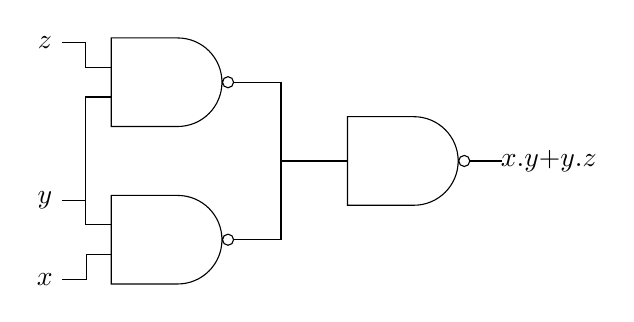
\begin{tikzpicture}[ circuit symbol wires]
    
    \node (x) at (0,0) {$x$};
    \node (y) at (0,1) {$y$};
    \node (z) at (0,3) {$z$};
    \node[nand gate US, minimum size=32pt, draw] at (1.5,0.5) (And) {};
    \node[nand gate US, minimum size=32pt, draw] at (1.5,2.5) (And1) {};
    \node[nand gate US, minimum size=32pt, draw] at (4.5,1.5) (And2) {};
    \draw (x.east) - ++(right:3mm) |- (And.input 2);
    \draw (y.east) - ++(right:3mm) |- (And.input 1);
    \draw (z.east) - ++(right:3mm) |- (And1.input 1);
    \draw (y.east) - ++(right:3mm) |- (And1.input 2);
    \draw (3.85,1.5) -- (3,1.5);
    \draw (3,0.5) -- (3,2.5);
    \draw (And.output) -- ($(And) + (1.5,0)$);
    \draw (And1.output) -- ($(And) + (1.5,2)$);
    \node (z) at ($(And2) + (1.9,0)$) {$x. y$+$y .z$};
    \draw (5.4,1.5) -- (5.8,1.5);
    
    \end{tikzpicture}
    \end{center}



\end{document}

